\documentclass[a4]{beamer}
\usepackage{amssymb}
\usepackage{graphicx}
\usepackage{subfigure}
\usepackage{newlfont}
\usepackage{amsmath,amsthm,amsfonts}
%\usepackage{beamerthemesplit}
\usepackage{pgf,pgfarrows,pgfnodes,pgfautomata,pgfheaps,pgfshade}
\usepackage{mathptmx}  % Font Family
\usepackage{helvet}   % Font Family
\usepackage{color}

\mode<presentation> {
 \usetheme{Default} % was Frankfurt
 \useinnertheme{rounded}
 \useoutertheme{infolines}
 \usefonttheme{serif}
 %\usecolortheme{wolverine}
% \usecolortheme{rose}
\usefonttheme{structurebold}
}

\setbeamercovered{dynamic}

\title[MathsCast]{Statistics for Computing \\ {\normalsize MA4413 Lecture 2A}}
\author[Kevin O'Brien]{Kevin O'Brien \\ {\scriptsize Kevin.obrien@ul.ie}}
\date{Autumn Semester 2013}
\institute[Maths \& Stats]{Dept. of Mathematics \& Statistics, \\ University \textit{of} Limerick}

\renewcommand{\arraystretch}{1.5}

\begin{document}

\begin{frame}
\titlepage
\end{frame}


%--------------------------------------------------------%

\begin{frame}
\frametitle{This Class}

\begin{itemize}
\item Notices: Change of Venues for classes
\item Descriptive Statistics: Sample Mean, Median and Variance
\item Descriptive Statistics: Inter-Quartile Range, Outliers and Skewness
\item Random Variables: Introduction at Random Variables
\end{itemize}

\end{frame}


%--------------------------------------------------------%
\frame{
\frametitle{Dispersion }

\begin{itemize}
\item The data values in a sample are not all the same. This variation between values is often called \textbf{ \emph{dispersion}}.

\item When the dispersion is large, the values are widely scattered; when it is small they are tightly clustered.

%The width of diagrams such as dot plots, box plots, stem and leaf plots is greater for samples with more dispersion and vice versa.

\item
There are several measures of dispersion, the most common being the variance and  standard deviation. These measures indicate to what degree the individual observations of a data set are dispersed or `spread out' around their mean.

\item
In engineering and science, high precision is associated with low dispersion.
\end{itemize}
}




%--------------------------------------------------------%
\frame{
\frametitle{Range}

\begin{itemize}
\item The range of a sample (or a data set) is a measure of the spread or the dispersion of the observations. \item It is the difference between the largest and the smallest observed value of some quantitative characteristic and is very easy to calculate.

\item A great deal of information is ignored when computing the range since only the largest and the smallest data values are considered; the remaining data are ignored.

\item The range value of a data set is greatly influenced by the presence of just one unusually large or small value in the sample (outlier).
\end{itemize}

\textbf{Example}


The range of $\{65,73,89,56,73,52,47\}$ is $ 89-47 = 42$.

% If the highest score in a 1st year statistics exam was 98 and the lowest 48, then the range would be 98-48 = 50.

}


%--------------------------------------------------------%


\frame{
\frametitle{Introducing Variance}

Consider the three data sets $X$, $Y$ and $Z$
\begin{itemize}
\item $X= \{900,925,950,975,1025,1050,1075,1100 \}$
\item $Y=\{900,905,910,920,1080,1090,1095,1100\}$
\item $Z=\{900,985,990,995,1005,1010,1015,1100\}$
\end{itemize}

For each of the data sets, the following statements can be verified

\begin{itemize}
\item The mean of each data set is 1000
\item There are 8 elements in each data set
\item The minima and maxima are 900 and 1100 for each set
\item The range is 200.
\end{itemize}

From the plot on the next slide, notice how different the three data sets are in terms of dispersion around the mean value.

}

%--------------------------------------------------------%

\frame{
\frametitle{Introducing Variance}


\begin{center}
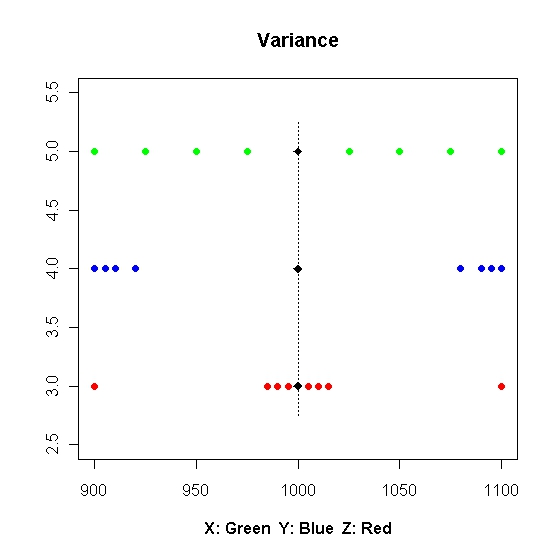
\includegraphics[scale=0.4]{2AVariance}
\end{center}

}

%--------------------------------------------------------%
\frame{
\frametitle{Variance}


\begin{itemize}

\item The (population) variance of a random variable is a non-negative number which gives an idea of how widely spread the values are likely to be; the larger the variance, the more scattered the observations on average.

\item Stating the variance gives an impression of how closely concentrated round the expected value the distribution is; it is a measure of the 'spread' of a distribution about its average value.

\item We distinguish between population variance (denoted $\sigma^2$) and sample variance (denoted $s^2$). Sample variance is simply the level of dispersion in a sample.For now, we will consider only at sample variance.

\end{itemize}

}


%-------------------------------------------------------------------------%
\frame{

\frametitle{Sample Variance}

\begin{itemize}

\item Sample variance is a measure of the spread of or dispersion within a set of sample data.

\item The sample variance is the sum of the squared deviations from their mean divided by one less than the number of observations in the data set.

\item For example, for $n$ observations $x_1, x_2, x_3, \ldots , x_n$  with sample mean $\bar{x}$, the sample variance is given by


 \[ s^2 = { \sum (x-\bar{x})^2  \over n-1}\]




\end{itemize}
}
%--------------------------------------------------%
\frame{
\frametitle{Sample Standard Deviation}
\begin{itemize}
\item \textbf{Important:} Standard deviation is the square root of variance
\item Standard deviation is commonly used in preference to variance because it is denominated in the same units as the mean.
\item For example, if dealing with time units, we could have a variance of something like $25$ \emph{ square minutes }, whereas the equivalent standard deviation is 5 minutes.
\item Population standard deviation is denoted  $\sigma$.
\item Sample standard deviation is denoted $s$.
\end{itemize}
}

%--------------------------------------------------------%
\begin{frame}[fragile]
\frametitle{Using \texttt{R}}Using \texttt{R} to compute standard deviation and variance for these data sets.

\begin{verbatim}
> X=c(900,925,950,975,1025,1050,1075,1100)
> Y=c(900,905,910,920,1080,1090,1095,1100)
> Z=c(900,985,990,995,1005,1010,1015,1100)
>
> sd(X);sd(Y);sd(Z)
[1] 73.19251
[1] 97.87018
[1] 54.37962
> 
>var(X);var(Y);var(Z)
[1] 5357.143
[1] 9578.571
[1] 2957.143
\end{verbatim}
\end{frame}
\frame{
\frametitle{Computing Sample Variance}
We shall use the following formulae to compute the sample variance of each data set (i.e. $s^2_x$, $s^2_y$ and $s^2_z$) respectively.

\[ s^2_x = { \sum (x-\bar{x})^2  \over n-1}\]
\[ s^2_y = { \sum (y-\bar{y})^2  \over n-1}\]
\[ s^2_z = { \sum (z-\bar{z})^2  \over n-1}\]
\begin{itemize}
\item Mean for each is 1000: $\bar{x} = \bar{y} = \bar{z}  = 1000$
\item Sample size of each data set is 8 : $ n=8 $
\item Therefore $ n-1 = 7$
\end{itemize}
}
%--------------------------------------------------%
\frame{
\frametitle{Computing Sample Variance}
\small
\[ s^2_x = {(900-1000)^2 +(925-1000)^2+ \ldots \ldots +(1075-1000)^2+(1100-1000)^2   \over 7}\]

\[ s^2_x = {(-100)^2 +(-75)^2 +(-50)^2+(-25)^2 + (25)^2 +(50)^2 +(75)^2+(100)^2   \over 7}\]

\[ s^2_x = {37500 \over 7}  = 5357.143\]

\normalsize
\bigskip The sample variance of $X$ is $5357.14$ square units. Recall that the sample standard deviation ($s$) is the square root of the variance, so for $X$  the sample standard deviation is $s_x = 73.19$ units.

}

%--------------------------------------------------%
\frame{
\frametitle{Computing Sample Variance}
Similarly \small
\[ s^2_y = {67050 \over 7}  = 9578.571 \mbox{ square units} \]

\[ s^2_z = {20700  \over 7} = 2957.143 \mbox{ square units} \]


\normalsize
\bigskip The sample standard deviations for $Y$ and $Z$ are $s_y = 97.87$ units, and $s_z =  54.38$ units respectively.
}



%----------------------------------------------------------%#

\frame{

\frametitle{Quartiles}

\begin{itemize}
\item Quartiles are values that divide a sample of data into four groups containing (as far as possible) equal numbers of observations.
\item
A data set has three quartiles. References to quartiles often relate to just the outer two, the upper and the lower quartiles; the second quartile being equal to the median. \item The lower quartile $Q_1$  is the data value a quarter way up through the ordered data set \item The upper quartile $Q_3$ is the data value a quarter way down from the highest value in an ordered data set.
\end{itemize}
}

%----------------------------------------------------------%#

\frame{

\frametitle{Computing Quartiles}
\begin{itemize}
\item Previously we discussed how to compute the median for odd-sized and even-sized data sets respectively (i.e. middle value or average of middle pair of values)
\item To compute $Q1$ and $Q3$, it is best to consider them as the median of the lower half of values and higher half of values respectively. \bigskip
\item Consider the following data set (ordered with 10 items):  $\{ 6, 7 ,15, 36, 39, 41, 41 ,43, 43, 47 \}$
\item The lower half of the data set is : $\{ 6, 7 ,15, 36, 39 \}$
\item The upper half of the data set is : $\{ 41, 41 ,43, 43, 47 \}$
\end{itemize}
}
%----------------------------------------------------------%#

\frame{

\frametitle{Computing Quartiles}
\begin{itemize}
\item For both the lower and upper halves, there is an odd number of items contained.
\item Recall that the median of the odd-sized data set is the middle value of the ordered set.
\item The medians are 15 and 43 respectively.
\item So the first and third quartiles are $Q_1 = 15$ and $Q_3 = 43$ respectively.
\end{itemize}
}

%----------------------------------------------------------%#

\frame{
\frametitle{Computing Quartiles}
In the last example, the full data set comprised an even number of items, and it was easy to split it into an lower half and an upper half. Consider the following data set.
\begin{itemize}
\item Data:  $\{6, 47, 49, 15, 43, 41, 7, 39, 43, 41, 36\}$
\item Ordered Data: $\{ 6, 7 ,15, 36, 39, 41, 41 ,43, 43, 47, 49 \}$
\item Sample size: 11
\item Median:  41 (6th item)
\end{itemize}
How do we split up the ordered data into two halves here?
}
%----------------------------------------------------------%#

\frame{
\frametitle{Computing Quartiles}
\begin{itemize}
\item The lower half of values  \begin{itemize} \item[A] - could contain either the lowest 5 values (i.e. excluding the median)

    \[\{ 6, 7 ,15, 36, 39\}\]
    \item[B] - or the lowest six values (i.e. including the median).  \[\{ 6, 7 ,15, 36, 39,41\}\] \end{itemize}
\item Consequently the upper half of values \begin{itemize} \item[A] -  will contain either the highest 5 values (i.e. excluding the median) \[\{ 41 ,43, 43, 47, 49 \}\] \item[B] - or the highest 6 values (i.e. including the median).
    \[\{ 41, 41 ,43, 43, 47, 49 \}\] \end{itemize}

\end{itemize}

}
%----------------------------------------------------------%#

\frame{
\frametitle{Computing Quartiles}
\begin{itemize}
\item The value of $Q_1$ and $Q_3$ depend on which approach is used to calculate them.
\begin{itemize}
\item For option $A$ : $Q_1 = 15$ and $Q_3 = 43$.
\item For option $B$ : $Q_1 = 25.5$ and $Q_3 = 43$.
\end{itemize}
\item Unfortunately there is no consensus on which approach to take; different textbooks use different approaches.
\item In some computing environments, different commands yields different results for quartiles.
\item For larger data sets, the difference in outcomes is often negligible.
\item In this module, we will use option $A$ (i.e. excluding the median) only.
\end{itemize}

}
%----------------------------------------------------------%#

\frame{
\frametitle{Interquartile Range}
\begin{itemize}
\item The interquartile range (IQR) is measure of dispersion, that can be used as an alternative to variance/standard deviation.
\item It is computed as follows:  \[ \mbox{ IQR }  = Q_3 - Q_1 \]
\item For the data set used previously:
 \[ \mbox{ IQR }  = 43 - 15  = 28 \]
\end{itemize}

}



%--------------------------------------------------------%
\frame{
\frametitle{Quantiles}
Quartiles are just one type of statistic known as ``Quantiles".
Quantiles are values which divide the distribution such that there is a given proportion of observations below the quantile.\\ \bigskip
\textbf{Other Examples of Quantiles}\\
\begin{description}
\item[Deciles]  any of the nine values that divide the sorted data into ten equal parts,
\item[Quintiles] any of the four values that divide the sorted data into five equal parts,
\item[Percentiles]any value below which a certain percentage of observations fall,
\end{description}

Quantiles can be expressed in terms of other quantiles. For example, the first decile is equivalent to the $10\%$ percentile, $Q_1$, the median and $Q_3$ are equivalent to the $25\%$, $50\%$, $75\%$ percentile.

}
%--------------------------------------------------------%
\frame{
\frametitle{Tukey five-number summary}
The Tukey five-number summary is a statistical summary that provides information about a dataset.
The summary consists of the five most commonly used sample quantiles:

\begin{itemize}
\item the lowest value in the dataset
\item the first quartile ($Q_1$)
\item the median ($Q_2$)
\item the third quartile ($Q_3$)
\item the highest value in the dataset
\end{itemize}

}

%-------------------------------------------------------------------------%

\section{Skewness and Outliers}

\frame{
\frametitle{Outliers}

\begin{itemize}
\item
An outlier is an observation in a data set which is far removed in value from the others in the data set. It is an unusually large or an unusually small value compared to the others.
\item
An outlier might be the result of an error in measurement, in which case it will distort the interpretation of the data, having undue influence on many summary statistics, for example, the mean and variance.
\item Outliers are said to \textbf{\emph{skew}} the distribution of values.
\item
If an outlier is a genuine result, it is important because it might indicate an extreme of behaviour of the process under study. \item For this reason, all outliers must be examined carefully before embarking on any formal analysis. Outliers should not routinely be removed without further justification.
\end{itemize}
}

%-------------------------------------------------------------------------%
\frame{
\frametitle{Outliers}
Compute the sample mean and median of the following data set
\[X = \{ 5, 6, 7, 8 ,9,11, 15, 16, 94\}\]

\begin{itemize}
\item The sample mean $\bar{x} = 19$
\item The median of the sample is 9.
\item What causes the discrepancy between mean and median?

\item Which measure of centrality do you feel is more representative of the data?
\begin{itemize}
\item The median  - most values are between 5 and 16.
\end{itemize}
\end{itemize}
}

%-------------------------------------------------------------------------%
\frame{
\frametitle{Symmetric and Skewed Distributions }
\begin{itemize}
\item  A data set is said to be \textbf{\emph{symmetric}} when data values are distributed in the same way above and below the middle of the sample.
\item Typically , but not necessarily, distributions are considered to symmetric because the data set does not contain any outliers. (Potentially a symmetric data set may contain outliers on either side of the mean. )
\item When data sets are symmetrically distributed, the sample mean and median have values close to each other.
\item Distributions are considered to \textbf{\emph{skewed}} when the data set contains an outlier, or cluster of outliers, distributed away from the main cluster of items, such as in our example.
\item When data sets have skewed distribution, the sample mean and median have values different to each other.
\end{itemize}
}
%-------------------------------------------------------------------------%
\frame{
\frametitle{Symmetric and Skewed Distributions }
\begin{itemize}
\item When a data set is \textbf{\emph{symmetric}}, the best measure of centrality is the sample mean.
\item As the variance is computed using the sample mean, it is considered the best measure of dispersion for symmetrically distributed data. \bigskip
\item When a data set is \textbf{\emph{skewed}}, the best measure of centrality is the median.
\item The best measure of dispersion for data with skewed distribution is the IQR.
\end{itemize}
}

%------------------------------------------------------------%
\frame{
\frametitle{Random Variables}
\begin{itemize} \item The outcome of an experiment need not be a number, for example, the outcome when a coin is tossed can be `heads' or `tails'. \item
However, we often want to represent outcomes as numbers. \item
A \textbf{\emph{random variable}} is a function that associates a unique numerical value with every outcome of an experiment.
\item The value of the random variable will vary from trial to trial as the experiment is repeated.
\item Numeric values can be assigned to outcomes that are not usually considered numeric. \item For example, we could assign a `head' a value of $0$, and a `tail' a value of $1$, or vice versa.
\end{itemize}
}
%------------------------------------------------------------%
\frame{
\frametitle{Random Variables}
There are two types of random variable - discrete and continuous. The distinction between both types will be important later on in the course.\\ \bigskip

\textbf{Examples}
\begin{itemize}
\item A coin is tossed ten times. The random variable X is the number of tails that are noted.
X can only take the values $\{0, 1, ..., 10\}$, so $X$ is a discrete random variable.
\item A light bulb is burned until it burns out. The random variable Y is its lifetime in hours.
Y can take any positive real value, so Y is a continuous random variable.
\end{itemize}
}

%--------------------------------------------------------------------------------%
\frame{
\frametitle{Discrete Random Variable}
\begin{itemize}
\item A discrete random variable is one which may take on only a countable number of distinct values such as $\{0, 1, 2, 3, 4, ... \}$ (i.e. a non-negative integer value).\item Discrete random variables are usually (but not necessarily) counts. \item If a random variable can take only a finite number of distinct values, then it must be discrete. \item Examples of discrete random variables include the number of children in a family, the Friday night attendance at a cinema, the number of patients in a doctor's surgery, the number of defective light bulbs in a box of ten.
    \end{itemize}
}


%--------------------------------------------------------------------------------%
\frame{
\frametitle{Continuous Random Variable}
\begin{itemize} \item
A continuous random variable is one which takes an infinite number of possible values 9 (i.e. a non-negative real number). \item Continuous random variables are usually measurements. \item Examples include height, weight, the amount of sugar in an orange, the time required to run a computer simulation. \end{itemize}

}

\section{Random Variables: Expected Value and Variance}

%--------------------------------------------------------%
\frame{

\frametitle{Expected Value for Discrete Random Variables}

\begin{itemize}

\item Consider the experiment of throwing a die repeatedly, where a record is kept of the mean score of all dice throws.
\item As the number of throws of the die increases, this average value will converge towards a specific value ( which is 3.5).
\item This value is the \textbf{\emph{expected value}} of all throws of a die.
\end{itemize}
}
%----------------------------------------------------------------%
\frame{
\frametitle{Expected Value for Discrete Random Variables}

\textbf{Previously}

Suppose we roll a die 8 times and get the following scores: $x = \{ 5, 2, 1, 6, 3, 5, 3, 1\}$ \\ \bigskip

What is the sample mean of the scores $\bar{x}$?
\[ \bar{x}  = {5 + 2 +  1 +  6 +  3 +  5 +  3 +  1 \over 8 } = {26 \over 8} =  3.25 \]

Suppose we roll the dice a further 4 times, yielding $\{ 5, 6, 1, 4 \}$, what is the sample mean then?

\[ \bar{x}  = {5 + 2 +  1 +  6 +  3 +  5 +  3 +  1  + 5 + 6 + 1 + 3 \over 12 } = {41 \over 12} =  3.416 \]
}
%--------------------------------------------------------%

\frame{
\frametitle{Expected Value for Discrete Random Variables}
\begin{itemize}
\item As the number of throws increases, the average value will start to settle around a particular value.
\item On the plot on the following slide we can see this convergence.
\item The red line indicates the values of sample mean of throws as the number of throws increases.
\item The green line indicates the level to which the mean value will converge to.
\end{itemize}

}
%--------------------------------------------------------%


\begin{frame}[fragile]
\frametitle{Dice Simulation in \texttt{R}}
\begin{verbatim}
> #simulate 10 rolls of a die
> n = 10
> x = sample(1:6,n,replace=TRUE)
> x
 [1] 5 1 4 2 6 6 2 4 2 5
>
> #Compute the cumulative average
> cumsum(x)/1:n
[1] 5.00 3.00 3.33 3.00 3.60 4.00 3.71 3.75 3.56 3.70
> 
\end{verbatim}
We will return to sampling at a later date. Meanwhile, you can try out this code for larger values of $n$.
\end{frame}

%--------------------------------------------------------%
\frame{
\frametitle{Expected Value for Discrete Random Variables}

\begin{center}
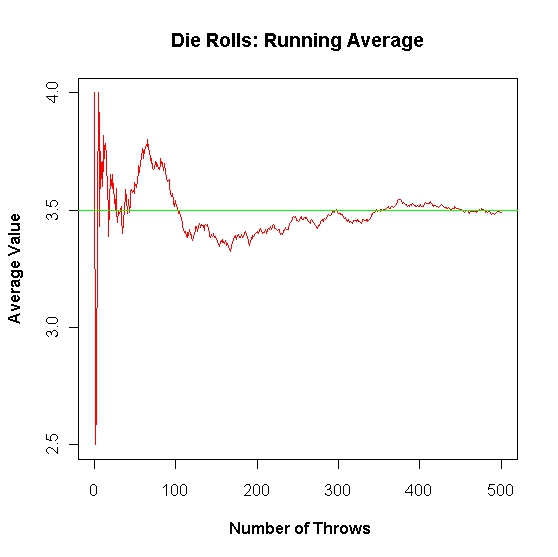
\includegraphics[scale=0.4]{2BDieMean}
\end{center}

}
%--------------------------------------------------------%
\frame{
\frametitle{Thought Experiment}

\begin{itemize}
\item Suppose you roll a die 100 times. You record the outcome for each roll, and compute the sum of the 100 rolls at the end.
\item What sum do you expect to end up with?
\item The lowest sum that is mathematically possible is 100. The highest is 600. To get either of these, you would have to roll the same number (either 1 or 6) 100 times in a row. Very unlikely ( but not impossible).
\item Instead you would expect to end up half way between 100 and 600, i.e. 350.
\item Every roll of a die should be worth 3.5 on average to your overall score.
\end{itemize}
}
%--------------------------------------------------------%

\frame{

\frametitle{Expected Value for Discrete Random Variables}

\begin{itemize}
\item The expected value of a discrete random variable $X$ is symbolized by E(X).

\item If X is a discrete random variable with possible values $\{ x_1, x_2, x_3,\ldots , x_n\}$, and $p(x_i)$ denotes $P(X = x_i)$, then the expected value of $X$ is defined by:

\[
E(X) = \sum x_i \times p(x_i)
\]

where the elements are summed over all values of the random variable $X$.

\end{itemize}

\textbf{Remark: } Expected values for continuous random variables are defined, but are not part of this module.
}
%--------------------------------------------------------%
\frame{
\frametitle{Expected Value for Discrete Random Variables}
When a die is thrown, each of the possible sides 1, 2, 3, 4, 5, 6 (i.e. the $x_i$ 's) has a
probability of 1/6 (the $p(x_i)$ s) of showing.
\\ \bigskip
The expected value of the face showing is therefore:

\[E(X) = (1 \times 1/6) + (2 \times 1/6) + (3 \times 1/6) + (4 \times 1/6) + (5 \times 1/6) + (6 \times 1/6)\]

\[E(X) = 21/6 = 3.5 \]
\bigskip
Notice that, in this case, $E(X)$ is $3.5$, which is not a possible value of X.


}
%--------------------------------------------------------%
\frame{
\frametitle{Expected Value for Discrete Random Variables}

Suppose we are playing a game where the points scored in each round are the square of the value shown by the die?
What is expected value of the score for each round.
\\ \bigskip
As we have defined a random variable $X$ to represent the number shown by each roll, we will define another $X^2$ to represent the points accrued by each roll.
\\ \bigskip
The expected value can be computed as follows:
\[
E(X^2) = \sum (x_i^2) \times p(x_i)
\]
}
%--------------------------------------------------------%
\frame{
\frametitle{Expected Value for Discrete Random Variables}
The expected value of the points is therefore:

\[E(X^2) = (1^2 \times 1/6) + (2^2 \times 1/6) + (3^2 \times 1/6) + (4^2 \times 1/6) + (5^2 \times 1/6) + (6^2 \times 1/6)\]

\[E(X^2) = 91/6 = 15.16 \]


}






%--------------------------------------------------------%
\frame{
\frametitle{Variance of a Discrete Random Variable}
We may require to know the variance of the random variable.

The variance of the random variable X, denoted $V(X)$, is defined to be:
\[ V(X) = E(X^2) - E(X)^2 \]
where $E(X)$ is the expected value of the random variable X.
}


%--------------------------------------------------------%
\frame{
\frametitle{Variance of a Discrete Random Variable}
Compute the variance for outcomes of the throws of a die, using
\[ V(X) = E(X^2) - E(X)^2 \].

We know that \begin{itemize} \item $E(X) = 21/6$ , so  $E(X)^2 = 441/36$. \\

\item $E(X^2)  = 91/6  = 546/36$

\item Therefore $V(X) = 546/36 - 441/36 = 105/36 = 2.91$
\end{itemize}

}
\end{document}


